\documentclass[12pt,a4paper,faculty=ea,language=en,doctype=report]{ugent-doc}
\geometry{bottom=2.5cm,top=2.5cm,left=2.5cm,right=2.5cm} 
\renewcommand{\baselinestretch}{1.15}

\usepackage{fontspec}
\setmainfont[
  ItalicFont=SourceSerifPro-LightItalic.ttf
]{SourceSerifPro-Light.ttf}
\setsansfont{WorkSans-Regular.ttf}
\usepackage[english]{babel}
% \usepackage{libertine}
% \usepackage{libertinust1math}
\usepackage{amsmath} % math equations

% code snippets
\setmonofont[
  ItalicFont=SourceCodePro-Italic.ttf,
  BoldFont=SourceCodePro-SemiBold.ttf,
]{SourceCodePro-Regular.ttf}
\usepackage{listings}

% transcriptions:
\usepackage{xparse}
\usepackage{enumitem}

% acronyms
\usepackage[printonlyused,withpage]{acronym}

% figures
\usepackage{graphicx} 
\usepackage{changepage}
\usepackage{pgfplots}
\graphicspath{{./figures/}}

% Bibliography
\usepackage[backend=biber, style=apa, sorting=nyt, hyperref=true]{biblatex} 
\addbibresource{references.bib}
\usepackage{csquotes} % Suggested when using babel+biblatex

% Ugent specific
\usepackage[colorlinks=true, allcolors=ugentblue]{hyperref} % Hyperreferences
\usepackage[parfill]{parskip} % Whitespace between paragraphs and no indentation

% code snippets
\usepackage{listings}
\usepackage{minted}
\usepackage{caption}
\captionsetup{justification=centering, margin=2cm}
\definecolor{mygray}{rgb}{0.95, 0.95, 0.95}
\definecolor{codeBlue}{rgb}{0.16, 0.22, 0.69}
\definecolor{codeGreen}{rgb}{0.16, 0.6, 0.44}
\setminted{
  breaklines=true,
  breakanywhere=true,
  fontsize=\footnotesize,
  bgcolor={mygray},
  style=lovelace
}
\makeatletter
\def\dontdofcolorbox{\renewcommand\fcolorbox[4][]{##4}}
\makeatother
\dontdofcolorbox

% styling table of contents
% \setcounter{tocdepth}{4}
\setcounter{secnumdepth}{4}

% hbox warning margin
\hfuzz=2pt

% for diagrams using Mathcha
\usepackage{tikz}
\usepackage{pgf-umlsd}
\usepgflibrary{arrows} % for pgf-uml

% for tables
\usepackage{booktabs}

% ---------------------------------------------

\thesubtitle{Linked Data}
\usepackage{ulem} % for colored underline
\renewcommand{\ULthickness}{2pt} % adjust thickness of underline
\thetitle{\uline{\color{ugentblue} Pre-culling geometric linked building data\\ for lightweight viewers}}
\infoboxa{\bfseries\large Master's dissertation submitted in order to obtain the academic degree of \\
Master of Science in de ingenieurswetenschappen: architectuur
}
\infoboxb{Supervisor: 
\begin{tabular}[t]{lll}
    Prof.\ ir.-arch.\ Paulus Present\\ % note syntax 'short space'
\end{tabular}
}
\infoboxc{Counselors: 
\begin{tabular}[t]{lll}
    Ir.-arch.\ Jeroen Werbrouck\\ % note syntax 'short space'
    Prof.\ dr.\ ir.\ arch.\ Ruben Verstraeten
\end{tabular}
}

\infoboxd{Philippe Soubrier 01702837 philippe.soubrier@ugent.be}
\infoboxe{Academic year: 2022--2023}

% ---------------------------------------------
\begin{document}
\maketitle
\renewcommand{\ULthickness}{1pt}
\normalem
\counterwithin{listing}{chapter}
% hide link color in toc and list of figures
{\hypersetup{hidelinks}
  \tableofcontents
  \listoffigures
  \let\clearpage\relax
  \listoftables
}

\newpage

\chapter*{Short abstract}
This is my short abstract.
\chapter*{Abstract}
This is my abstract
\chapter{Introduction}
\section{Context}
\subsection{3D viewers}
-> Applications?

-> Who uses them?

-> What for?

\subsection{\acs{bim} geometry} \label{subsec:bimGeometry}
% -> What is \ac{bim}? (short)

% -> Extend of \ac{bim} geometry?
% -> Complexity of \ac{bim} geometry?
The 3D model of a building consists of a multitude of sub-models, describing objects for all the different stakeholders participating to the porject. Some describe very large objects, and some very small parts. Both can be defined in there most simple and abstract form or have an intricate and complex geometry. As a basic example, can a door simply be defined as a box, or up to the level of the screw-thread for the hinge system. The level of abstraction is here described as the \ac{lod} and is most of the time pre-selected for the needs of a \ac{bim} model, and is applied throughout a single model.

\begin{figure}
    \centering
    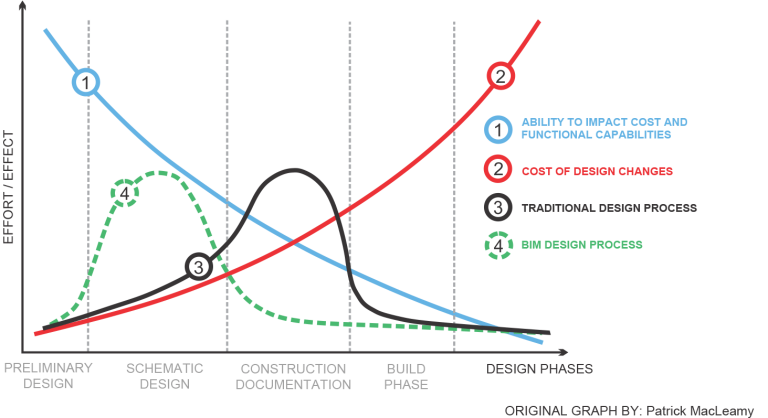
\includegraphics[width=0.5\textwidth]{figures/BIM grafiek.png}
    \caption{Evolution of \ac{lod} during the life-cycle of a building.}
    \label{fig:bimGraph}
\end{figure}

As shown in figure~\ref{fig:bimGraph}, a standard BIM workflow goes through multiple fases each with there assosiated model and \ac{lod}. The \ac{lod} is a very important concept in the \ac{aec} industry, as it allows for a very efficient workflow. Approaching the modeling step from a top-down perspective, starting with rougher geometries descriving the rougher ideas of a concept model and evoluting to a more refined model for the construction fase. As last and longest standing model, can a higher \ac{lod} be used to describe suttle changes in the evolution of a building.

This amount of data, both accounting for the \\
-> Some data BB models

\subsection{\acs{ldbim}}
% -> ! Focus on geometry

% -> What is \ac{ldbim}?

% -> Why the need / What are the advantages of \ac{ldbim}?

% -> Context od enrichment and complexity

-> Own definition of \ac{ldbim}

The interconnectivity of semantics can also be applied to geometry descriptions. Which could allow the co-existance of multiple \ac{lod}'s in a single model. Besides storing the evolution of an single element's geometry, it allows the linking of the different \ac{lod}'s to each other. In contrary to a standard \ac{bim} models, as explained in \ref{subsec:bimGeometry}.

\subsection{Computing power dilemma}
The enrichment of the \ac{ldbim}-graph also comes with a cost. The amount of data that needs to be stored and processed is much larger than a standard \ac{bim} model. Viewers greatly suffer from enrichment as most standard applications require the full model to be loaded in memory.

-> What is the hardware problem?

-> Why is it that important for the \ac{aec} industry?

\section{Research questions}

-> Why the need for this thesis? (why a \ac{ldbim} viewer?)

-> What is the possible solution? (Culling algorithms)

-> Why the need for research questions?
(culling algorithms are not new, always progress, see later)

\subsection[Can \acs{ldbim} be culled?]{To which extent can \acs{ldbim} geometry be culled\\
    to be streamed to lightweight viewers?}
-> What can be culled exactly?

-> What needs to be streamed?

-> What is the impact of culling on the viewing experience?

\subsection[Can existing semantic be used?]{Can existing semantic and ontologies be used to\\
    feed possible culling algorithms?}
-> What are ontologies?

-> Can GIS ontologies be used too?

-> What are the advantages of using ontologies?

\section{Research objectives}
\subsection[Advantages of LDBIM]{Bring forward the advantages of \acs{ldbim} for visualization of big 3D models}
-> Showcase that existing models are already mature enough for these usecases.

->
\subsection[Showcase the fisability]{Showcase the fisability of \acs{ldbim} for visualization of big 3D models}
->
\chapter{State of the art}
As mentioned in \cite{Johansson2015}, existing research on the performance of currently used \ac{bim} viewers is quite limited. This state-of-the-art research will, therefore, focus on the overall features of some promising newer viewers and the ontologies that will be used in this thesis.

\section{Existing \acs{bim} viewers and ontologies}
\subsection{Qoniq and \acs{lod} Streaming for \acs{bim}}
Qonic focuses on developing an open platform \ac{bim} viewer. With the use of Unity to enable cross-platform compatibility, they focused on two main aspects: performance and aesthetics. The latter refers to the visual quality of the viewer, offering both a seamless experience for the viewer as well as a pleasant one, with, for example, the implementation of ambient lighting and shadow castings. The first and most researched aspect of their viewer, the performance, is mainly focusing on a \ac{lod} culling algorithm.
\\(T. Strobbe, personal communication, November 25, 2022)

\subsubsection{Qoniq's approach to \acs{lod} streaming}
Their core research is developing a dynamic \ac{lod} streaming model. Starting from the geometry and semantics of an \ac{ifc} file, they compute an \ac{lod} hierarchy tree of the model. Through multiple mesh decimation algorithms, they reduce the number of triangles of each object's mesh, regardless of the semantics associated with that object. On top of that, a filtering algorithm is implemented in the streaming model to filter out objects, regarding their semantics, that are not relevant to the current camera position. In doing so, they both reduce the size of models far from the viewpoint and evaluate the need to show certain objects based on their nature, extracted from semantics in the \ac{ifc} file, and their distance to the camera. The resulting dynamic \ac{lod} streaming model is reevaluated at each camera move in Unity.
\\(T. Strobbe, personal communication, November 25, 2022)

Unity was chosen as it allows for writing once and deploying everywhere. This means that the viewer can be used on any platform, including mobile devices and browsers. The performance results are thus related to the hardware capabilities of each device, with the exception of the browser, where the performance of Unity's WebGL build is limited to a scene size of 2Gb.\footcite{UnityWebGL}

\subsubsection{Advantages and trade-offs}
Being able to run on many platforms, offering a smooth viewer experience and a pleasing aesthetic makes it an ideal candidate for lightweight viewers on the job site. However, the \ac{lod} library has to be computed on every model update. The decimation algorithms are furthermore computational results that are not humanly reviewed. This means that the quality of the resulting meshes is not guaranteed for the lower \ac{lod}s, which are, as illustrated in Figure \ref{fig:bimGraph}, already modeled in previous design phases. \ac{ldbim} could, by interconnection, recall previous \ac{lod}s in the viewer's scene. Without the need for computational remodeling. Nevertheless, Qonic serves as this thesis's goal, outside the \ac{ldbim} context.

\subsection{ld-bim.web.app}
\enquote{The purpose of the app is to showcase our LBD toolset and to demonstrate the capabilities of Linked Building Data to newcomers.} \footcite{lbdimApp}

\url{https://ld-bim.web.app/} demonstrates a viewer built around an \ac{rdf} database. It separates the data from an \ac{ifc} file into semantics, stored in the previously mentioned graph, and a glTF model, together with a \ac{json} file containing a reference table. Extra local or remote graphs can be added to the \ac{ui}. As it contains a \ac{sparql} engine to query and visualize, in the form of highlighting, the results of the query in a 3D viewer. The viewer is based on the ifc.js project, which is itself based on the three.js 3D JavaScript library.

\subsection{\acs{aec} related ontologies}
As mentioned in the second research question \ref{subsec:rq2}, this section will discuss \ac{aec}-related technologies, some of which are not yet approved by the \ac{w3c} but are actively researched by the \ac{lbd-cg}\footcites{lbdOntologies}

\subsubsection{\acs{bot}}
The \ac{bot} proposes a set of classes and properties, \enquote{which provides a high-level description of the topology of buildings including storeys and spaces, the building elements they may contain, and the 3D mesh geometry of these spaces and elements.} \parencite{Rasmussen2020}, as illustrated in Figure \ref{fig:bot}. This high-level description could be fed to portal-culling algorithms in a situation where the visibility is contained within one \mintinline{turtle}|bot:Space| or \mintinline{turtle}|bot:Storey|, or it could extend the scope to \mintinline{turtle}|bot:adjacentZone|\footcite{GodotPortal}. Additionally, it could play a part in the construction of the \ac{bvh} needed for other occlusion culling algorithms, such as the \ac{chc}++ \parencite{Johansson2015}.

\begin{figure}[H]
    \begin{adjustwidth}{-0.8cm}{-0.8cm}
        \centering
        

\tikzset{every picture/.style={line width=0.75pt}} %set default line width to 0.75pt        

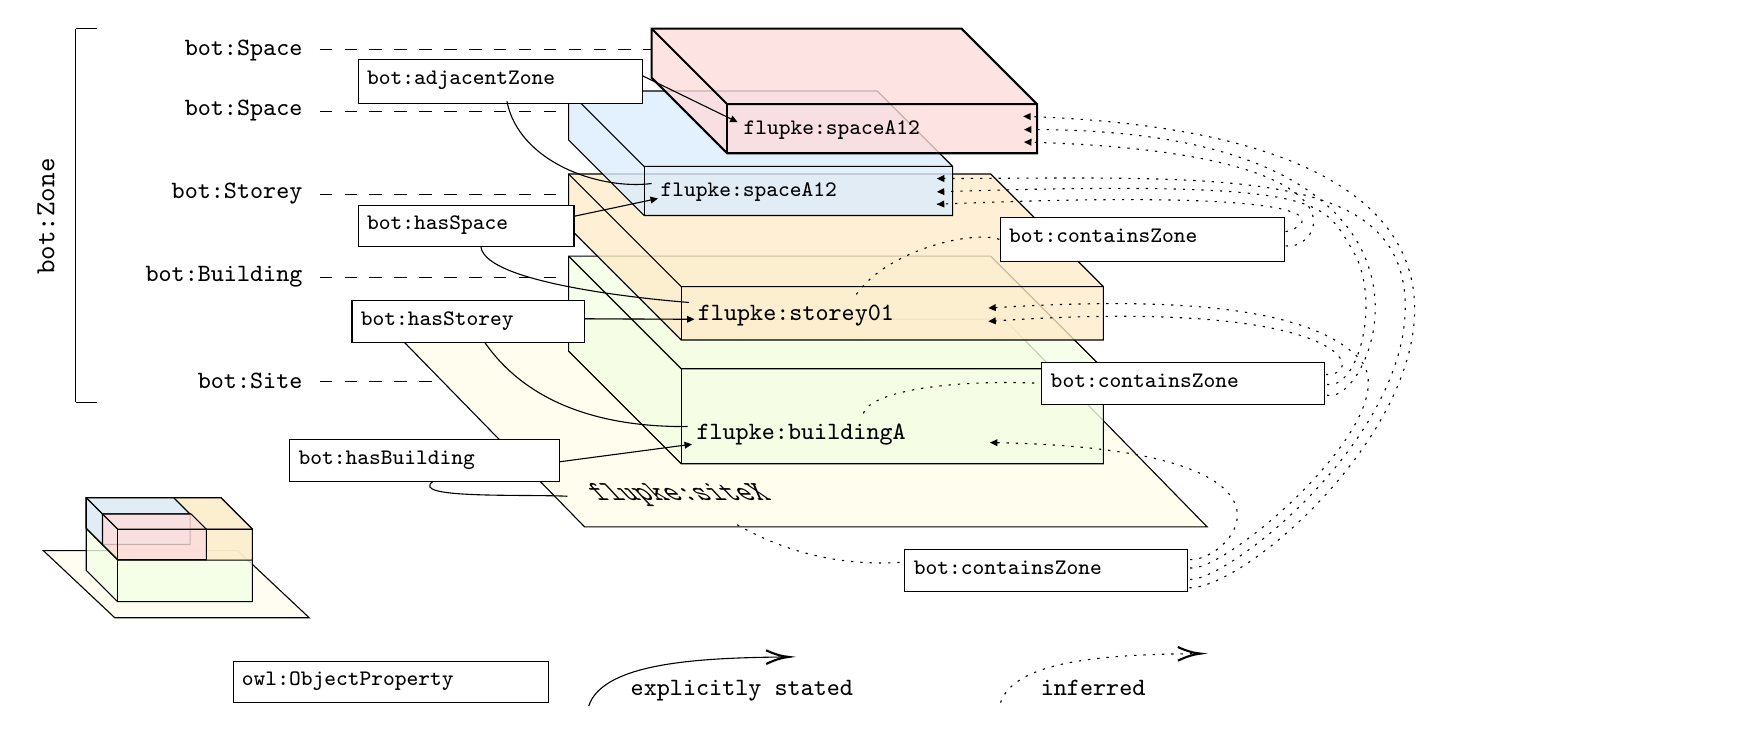
\begin{tikzpicture}[x=0.75pt,y=0.75pt,yscale=-1,xscale=1]
    \ttfamily
%uncomment if require: \path (0,373); %set diagram left start at 0, and has height of 373

%Shape: Parallelogram [id:dp6234888353745478] 
\draw  [fill={rgb, 255:red, 255; green, 253; blue, 237 }  ,fill opacity=0.8 ] (113,261.47) -- (19.33,261.47) -- (53.73,293.8) -- (147.4,293.8) -- cycle ;
%Shape: Parallelogram [id:dp5369889401184471] 
\draw  [fill={rgb, 255:red, 255; green, 253; blue, 237 }  ,fill opacity=1 ] (482.33,150) -- (182.41,150) -- (280.07,250) -- (580,250) -- cycle ;
%Shape: Cube [id:dp8255469967169493] 
\draw  [fill={rgb, 255:red, 243; green, 255; blue, 228 }  ,fill opacity=0.8 ] (530,173.85) -- (475.75,119.6) -- (272.41,119.6) -- (272.41,165.35) -- (326.66,219.6) -- (530,219.6) -- cycle ; \draw   (272.41,119.6) -- (326.66,173.85) -- (530,173.85) ; \draw   (326.66,173.85) -- (326.66,219.6) ;
%Shape: Cube [id:dp7451550676115966] 
\draw  [fill={rgb, 255:red, 254; green, 235; blue, 202 }  ,fill opacity=0.8 ] (530,134.25) -- (475.75,80) -- (272.41,80) -- (272.41,105.75) -- (326.66,160) -- (530,160) -- cycle ; \draw   (272.41,80) -- (326.66,134.25) -- (530,134.25) ; \draw   (326.66,134.25) -- (326.66,160) ;
%Shape: Cube [id:dp7376474366082748] 
\draw  [fill={rgb, 255:red, 220; green, 236; blue, 254 }  ,fill opacity=0.8 ] (457.41,76.33) -- (421.07,40) -- (272.41,40) -- (272.41,63.67) -- (308.74,100) -- (457.41,100) -- cycle ; \draw   (272.41,40) -- (308.74,76.33) -- (457.41,76.33) ; \draw   (308.74,76.33) -- (308.74,100) ;
%Shape: Cube [id:dp6037678452495017] 
\draw  [fill={rgb, 255:red, 254; green, 220; blue, 220 }  ,fill opacity=0.8 ][line width=0.75]  (498.07,46.33) -- (461.74,10) -- (312.41,10) -- (312.41,33.67) -- (348.74,70) -- (498.07,70) -- cycle ; \draw  [line width=0.75]  (312.41,10) -- (348.74,46.33) -- (498.07,46.33) ; \draw  [line width=0.75]  (348.74,46.33) -- (348.74,70) ;
%Curve Lines [id:da34503747339894364] 
\draw  [dash pattern={on 0.84pt off 2.51pt}]  (617.81,114.6) .. controls (634.52,117.78) and (665.49,69.49) .. (494.4,64.67) ;
\draw [shift={(491.81,64.6)}, rotate = 1.45] [fill={rgb, 255:red, 0; green, 0; blue, 0 }  ][line width=0.08]  [draw opacity=0] (3.57,-1.72) -- (0,0) -- (3.57,1.72) -- cycle    ;
%Curve Lines [id:da8352390399084118] 
\draw  [dash pattern={on 0.84pt off 2.51pt}]  (617.81,107.8) .. controls (628.61,105.4) and (659.41,85.8) .. (449.81,94.6) ;
\draw [shift={(449.81,94.6)}, rotate = 357.6] [fill={rgb, 255:red, 0; green, 0; blue, 0 }  ][line width=0.08]  [draw opacity=0] (3.57,-1.72) -- (0,0) -- (3.57,1.72) -- cycle    ;
%Curve Lines [id:da4764695659197302] 
\draw  [dash pattern={on 0.84pt off 2.51pt}]  (637.81,186.6) .. controls (660.61,192.6) and (716.61,57) .. (491.81,58.6) ;
\draw [shift={(491.81,58.6)}, rotate = 359.59] [fill={rgb, 255:red, 0; green, 0; blue, 0 }  ][line width=0.08]  [draw opacity=0] (3.57,-1.72) -- (0,0) -- (3.57,1.72) -- cycle    ;
%Curve Lines [id:da6997716856913325] 
\draw  [dash pattern={on 0.84pt off 2.51pt}]  (637.81,181.4) .. controls (653.41,183.8) and (664.21,139.4) .. (649.81,116.2) .. controls (635.48,93.12) and (638.97,82.7) .. (452.63,88.51) ;
\draw [shift={(449.81,88.6)}, rotate = 358.18] [fill={rgb, 255:red, 0; green, 0; blue, 0 }  ][line width=0.08]  [draw opacity=0] (3.57,-1.72) -- (0,0) -- (3.57,1.72) -- cycle    ;
%Curve Lines [id:da2611543315656344] 
\draw  [dash pattern={on 0.84pt off 2.51pt}]  (637.21,176.6) .. controls (656.91,177.4) and (651.86,138.99) .. (477.25,150.82) ;
\draw [shift={(474.61,151)}, rotate = 356] [fill={rgb, 255:red, 0; green, 0; blue, 0 }  ][line width=0.08]  [draw opacity=0] (3.57,-1.72) -- (0,0) -- (3.57,1.72) -- cycle    ;
%Curve Lines [id:da3444743375210677] 
\draw  [dash pattern={on 0.84pt off 2.51pt}]  (571.41,279.4) .. controls (618.61,279.4) and (830.21,63.4) .. (491.41,52.2) ;
\draw [shift={(491.41,52.2)}, rotate = 1.89] [fill={rgb, 255:red, 0; green, 0; blue, 0 }  ][line width=0.08]  [draw opacity=0] (3.57,-1.72) -- (0,0) -- (3.57,1.72) -- cycle    ;
%Curve Lines [id:da00012227444950441146] 
\draw  [dash pattern={on 0.84pt off 2.51pt}]  (571.81,269.8) .. controls (588.81,272.6) and (679.01,195) .. (653.01,168.6) .. controls (627.27,142.46) and (556.83,139.46) .. (477.03,144.45) ;
\draw [shift={(474.61,144.6)}, rotate = 356.32] [fill={rgb, 255:red, 0; green, 0; blue, 0 }  ][line width=0.08]  [draw opacity=0] (3.57,-1.72) -- (0,0) -- (3.57,1.72) -- cycle    ;
%Curve Lines [id:da2737876317435528] 
\draw  [dash pattern={on 0.84pt off 2.51pt}]  (571.81,265.8) .. controls (591.51,266.6) and (641.3,212.35) .. (477.89,209.44) ;
\draw [shift={(475.41,209.4)}, rotate = 0.83] [fill={rgb, 255:red, 0; green, 0; blue, 0 }  ][line width=0.08]  [draw opacity=0] (3.57,-1.72) -- (0,0) -- (3.57,1.72) -- cycle    ;
%Curve Lines [id:da48651030268326223] 
\draw  [dash pattern={on 0.84pt off 2.51pt}]  (571.81,275.4) .. controls (591.47,275.4) and (678.21,205.8) .. (675.41,141) .. controls (672.62,76.52) and (587.07,81.75) .. (451.85,82.19) ;
\draw [shift={(449.81,82.2)}, rotate = 359.83] [fill={rgb, 255:red, 0; green, 0; blue, 0 }  ][line width=0.08]  [draw opacity=0] (3.57,-1.72) -- (0,0) -- (3.57,1.72) -- cycle    ;
%Straight Lines [id:da018272292431112502] 
\draw  [dash pattern={on 4.5pt off 4.5pt}]  (152.41,20) -- (312.41,20) ;
%Straight Lines [id:da7335835552603491] 
\draw  [dash pattern={on 4.5pt off 4.5pt}]  (152.41,50) -- (272.41,50) ;
%Straight Lines [id:da8480379890588858] 
\draw  [dash pattern={on 4.5pt off 4.5pt}]  (152.41,90) -- (272.41,90) ;
%Straight Lines [id:da5645617535440737] 
\draw  [dash pattern={on 4.5pt off 4.5pt}]  (152.41,130) -- (272.41,130) ;
%Straight Lines [id:da7578549164754749] 
\draw  [dash pattern={on 4.5pt off 4.5pt}]  (152.41,180) -- (212.41,180) ;
%Straight Lines [id:da4046157540132602] 
\draw    (35,10) -- (35,190) ;
%Straight Lines [id:da9585577369264056] 
\draw    (35,10) -- (45,10) ;
%Straight Lines [id:da8679205527736427] 
\draw    (35,190) -- (45,190) ;
%Straight Lines [id:da4346199951984231] 
\draw    (265.4,219) -- (328.83,210.59) ;
\draw [shift={(331.8,210.2)}, rotate = 172.45] [fill={rgb, 255:red, 0; green, 0; blue, 0 }  ][line width=0.08]  [draw opacity=0] (3.57,-1.72) -- (0,0) -- (3.57,1.72) -- cycle    ;
%Straight Lines [id:da9955272147380352] 
\draw    (275.7,149.72) -- (330,149.99) ;
\draw [shift={(333,150)}, rotate = 180.28] [fill={rgb, 255:red, 0; green, 0; blue, 0 }  ][line width=0.08]  [draw opacity=0] (3.57,-1.72) -- (0,0) -- (3.57,1.72) -- cycle    ;
%Straight Lines [id:da5290759611186164] 
\draw    (268.7,101.72) -- (312.47,92.42) ;
\draw [shift={(315.4,91.8)}, rotate = 168.01] [fill={rgb, 255:red, 0; green, 0; blue, 0 }  ][line width=0.08]  [draw opacity=0] (3.57,-1.72) -- (0,0) -- (3.57,1.72) -- cycle    ;
%Straight Lines [id:da2082247372760495] 
\draw    (307.8,32.6) -- (351.1,53.69) ;
\draw [shift={(353.8,55)}, rotate = 205.96] [fill={rgb, 255:red, 0; green, 0; blue, 0 }  ][line width=0.08]  [draw opacity=0] (3.57,-1.72) -- (0,0) -- (3.57,1.72) -- cycle    ;
%Shape: Cube [id:dp41271376617212563] 
\draw  [fill={rgb, 255:red, 243; green, 255; blue, 228 }  ,fill opacity=0.8 ] (120,251) -- (105,236) -- (40,236) -- (40,271) -- (55,286) -- (120,286) -- cycle ; \draw   (40,236) -- (55,251) -- (120,251) ; \draw   (55,251) -- (55,286) ;
%Shape: Cube [id:dp24709864473657217] 
\draw  [fill={rgb, 255:red, 254; green, 235; blue, 202 }  ,fill opacity=0.8 ] (120,251.17) -- (104.83,236) -- (40,236) -- (40,250.83) -- (55.17,266) -- (120,266) -- cycle ; \draw   (40,236) -- (55.17,251.17) -- (120,251.17) ; \draw   (55.17,251.17) -- (55.17,266) ;
%Shape: Cube [id:dp7279118293384432] 
\draw  [fill={rgb, 255:red, 220; green, 236; blue, 254 }  ,fill opacity=0.8 ] (90,243.83) -- (82.17,236) -- (40,236) -- (40,250.67) -- (47.83,258.5) -- (90,258.5) -- cycle ; \draw   (40,236) -- (47.83,243.83) -- (90,243.83) ; \draw   (47.83,243.83) -- (47.83,258.5) ;
%Shape: Cube [id:dp46117172286245767] 
\draw  [fill={rgb, 255:red, 254; green, 220; blue, 220 }  ,fill opacity=0.8 ] (97.83,251.17) -- (90.5,243.83) -- (47.83,243.83) -- (47.83,258.5) -- (55.17,265.83) -- (97.83,265.83) -- cycle ; \draw   (47.83,243.83) -- (55.17,251.17) -- (97.83,251.17) ; \draw   (55.17,251.17) -- (55.17,265.83) ;
%Curve Lines [id:da718845720785724] 
\draw    (282.08,336.27) .. controls (289.17,314.99) and (337.4,313.12) .. (376.69,312.69) ;
\draw [shift={(378.48,312.67)}, rotate = 179.42] [color={rgb, 255:red, 0; green, 0; blue, 0 }  ][line width=0.75]    (10.93,-3.29) .. controls (6.95,-1.4) and (3.31,-0.3) .. (0,0) .. controls (3.31,0.3) and (6.95,1.4) .. (10.93,3.29)   ;
%Curve Lines [id:da5183556614244442] 
\draw  [dash pattern={on 0.84pt off 2.51pt}]  (480.48,334.67) .. controls (487.57,313.39) and (535.8,311.52) .. (575.09,311.09) ;
\draw [shift={(576.88,311.07)}, rotate = 179.42] [color={rgb, 255:red, 0; green, 0; blue, 0 }  ][line width=0.75]    (10.93,-3.29) .. controls (6.95,-1.4) and (3.31,-0.3) .. (0,0) .. controls (3.31,0.3) and (6.95,1.4) .. (10.93,3.29)   ;

% Text Node
\draw (276.69,228) node [anchor=north west][inner sep=0.75pt]  [xslant=-0.93] [align=left] {flupke:siteX};
% Text Node
\draw (332.74,199.33) node [anchor=north west][inner sep=0.75pt]  [font=\small] [align=left] {flupke:buildingA \ \ \ \ \ \ \ \ \ \ };
% Text Node
\draw (333.41,142) node [anchor=north west][inner sep=0.75pt]  [font=\small] [align=left] {flupke:storey01 \ \ \ \ \ \ \ \ \ \ };
% Text Node
\draw (355.41,53) node [anchor=north west][inner sep=0.75pt]  [font=\footnotesize] [align=left] {flupke:spaceA12 \ \ \ \ \ \ \ \ \ \ };
% Text Node
\draw  [fill={rgb, 255:red, 255; green, 255; blue, 255 }  ,fill opacity=1 ]  (480.41,101) -- (617.41,101) -- (617.41,122) -- (480.41,122) -- cycle  ;
\draw (483.41,105) node [anchor=north west][inner sep=0.75pt]  [font=\footnotesize] [align=left] {bot:containsZone \ \ \ \ \ \ \ \ \ \ };
% Text Node
\draw  [fill={rgb, 255:red, 255; green, 255; blue, 255 }  ,fill opacity=1 ]  (500.41,171) -- (636.41,171) -- (636.41,191) -- (500.41,191) -- cycle  ;
\draw (503.41,175) node [anchor=north west][inner sep=0.75pt]  [font=\footnotesize] [align=left] {bot:containsZone \ \ \ \ \ \ \ \ \ \ };
% Text Node
\draw  [fill={rgb, 255:red, 255; green, 255; blue, 255 }  ,fill opacity=1 ]  (434.41,261) -- (570.41,261) -- (570.41,281) -- (434.41,281) -- cycle  ;
\draw (437.41,265) node [anchor=north west][inner sep=0.75pt]  [font=\footnotesize] [align=left] {bot:containsZone \ \ \ \ \ \ \ \ \ \ };
% Text Node
\draw (315.41,83) node [anchor=north west][inner sep=0.75pt]  [font=\footnotesize] [align=left] {flupke:spaceA12 \ \ \ \ \ \ \ \ \ \ };
% Text Node
\draw (145.41,20.5) node [anchor=east] [inner sep=0.75pt]  [font=\small] [align=left] {bot:Space};
% Text Node
\draw (145.41,49.5) node [anchor=east] [inner sep=0.75pt]  [font=\small] [align=left] {bot:Space};
% Text Node
\draw (145.41,89.5) node [anchor=east] [inner sep=0.75pt]  [font=\small] [align=left] {bot:Storey};
% Text Node
\draw (145.41,129.5) node [anchor=east] [inner sep=0.75pt]  [font=\small] [align=left] {bot:Building};
% Text Node
\draw (145.41,179.5) node [anchor=east] [inner sep=0.75pt]  [font=\small] [align=left] {bot:Site};
% Text Node
\draw (20.5,100.5) node  [font=\normalsize,rotate=-270] [align=left] {bot:Zone};
% Text Node
\draw  [fill={rgb, 255:red, 255; green, 255; blue, 255 }  ,fill opacity=1 ]  (138,208) -- (268,208) -- (268,228) -- (138,228) -- cycle  ;
\draw (141,212) node [anchor=north west][inner sep=0.75pt]  [font=\footnotesize] [align=left] {bot:hasBuilding \ \ \ \ \ \ \ \ \ \ \ };
% Text Node
\draw  [fill={rgb, 255:red, 255; green, 255; blue, 255 }  ,fill opacity=1 ]  (168,141) -- (280,141) -- (280,161) -- (168,161) -- cycle  ;
\draw (171,145) node [anchor=north west][inner sep=0.75pt]  [font=\footnotesize] [align=left] {bot:hasStorey \ \ \ \ \ \ \ \ };
% Text Node
\draw  [fill={rgb, 255:red, 255; green, 255; blue, 255 }  ,fill opacity=1 ]  (171,25) -- (308,25) -- (308,46) -- (171,46) -- cycle  ;
\draw (174,29) node [anchor=north west][inner sep=0.75pt]  [font=\footnotesize] [align=left] {bot:adjacentZone \ \ \ \ \ \ \ \ \ \ };
% Text Node
\draw  [fill={rgb, 255:red, 255; green, 255; blue, 255 }  ,fill opacity=1 ]  (171,95) -- (275,95) -- (275,115) -- (171,115) -- cycle  ;
\draw (174,99) node [anchor=north west][inner sep=0.75pt]  [font=\footnotesize] [align=left] {bot:hasSpace \ \ \ \ \ \ };
% Text Node
\draw  [fill={rgb, 255:red, 255; green, 255; blue, 255 }  ,fill opacity=1 ]  (110.74,314.83) -- (262.74,314.83) -- (262.74,334.83) -- (110.74,334.83) -- cycle  ;
\draw (113.74,318.83) node [anchor=north west][inner sep=0.75pt]  [font=\footnotesize] [align=left] {owl:ObjectProperty \ \ \ \ \ \ \ \ \ \ \ \ };
% Text Node
\draw (301.04,322.88) node [anchor=north west][inner sep=0.75pt]  [font=\small] [align=left] {explicitly stated};
% Text Node
\draw (498.64,322.88) node [anchor=north west][inner sep=0.75pt]  [font=\small] [align=left] {inferred};
% Connection
\draw  [dash pattern={on 0.84pt off 2.51pt}]  (353.59,249) .. controls (378.56,263.15) and (405.5,269.14) .. (434.41,266.98) ;
% Connection
\draw  [dash pattern={on 0.84pt off 2.51pt}]  (414.39,195.33) .. controls (417.83,184.2) and (459.52,178.83) .. (500.41,180.89) ;
% Connection
\draw  [dash pattern={on 0.84pt off 2.51pt}]  (411,138) .. controls (426.16,116.24) and (468.16,106.77) .. (480.41,111.68) ;
% Connection
\draw    (271.82,235.25) .. controls (248.39,234.24) and (195.05,236.49) .. (207.18,228) ;
% Connection
\draw    (329.74,201.67) .. controls (289.49,202.06) and (252.87,191.28) .. (231.88,161) ;
% Connection
\draw    (330.41,141.89) .. controls (315.58,140.78) and (232.01,133.24) .. (230.12,115) ;
% Connection
\draw    (312.41,84.59) .. controls (286.33,87.84) and (248.33,73.82) .. (242.66,45) ;

\end{tikzpicture}

        \vspace{-0.3cm}
        \caption[Illustration of the \acs{bot} ontology]{Illustration of the \acs{bot} ontology, based on \cite{Rasmussen2020}.}
        \label{fig:bot}
    \end{adjustwidth}
\end{figure}

\subsubsection{\acs{fog} and \acs{omg}}
With the help of \ac{fog} and \ac{omg}, geometry descriptions can be linked in the data graph. The innovation lies in the choice to store it either inside or outside the graph, by means of one triple referring to a literal or an \ac{uri}. Listing \ref{lst:rdfSample} showcases multiple examples of objects assigned with a geometry description using an \ac{uri}\parencite{Bonduel2019}.

\begin{listing}[H]
    \begin{minted}{turtle}
flupke:coneOBJ_geometry-1 fog:asObj_v3.0-obj "https://..."^^xsd:anyURI .
    \end{minted}
    \vspace{-0.7cm}
    \caption{Example of \acs{fog} usage}
    \label{lst:fogSample}
\end{listing}

Listing \ref{lst:fogSample} describes a subject of datatype \mintinline{turtle}|xsd:anyURI| from the \ac{xsd}\footcites{xsd}. The versatile approach of \cite{Bonduel2019} also proposes the following datatypes: \mintinline{turtle}|xsd:string| for \ac{ascii}-based geometry descriptions or \mintinline{turtle}|xsd:base64Binary| for binary geometry descriptions.

The format of the geometry is assigned directly by the predicate in Listing \ref{lst:fogSample}, which is \mintinline{turtle}|fog:asObj_v3.0-obj|. This further infers the statements in Listing \ref{lst:fogInference}.\footcite{fog}

\begin{listing}[H]
    \begin{minted}{turtle}
flupke:coneOBJ_geometry-1 fog:asObj "https://..."^^xsd:anyURI ;
    ex:LOD "100"^^xsd:integer .
    \end{minted}
    \vspace{-0.7cm}
    \caption{\acs{fog} inference examples}
    \label{lst:fogInference}
\end{listing}

\cite{Bonduel2019} refers to the proposal of the \ac{lbd-cg} stated in \cite{Wagner2019} \enquote{to allow the modeling of properties on three levels}. The first and second levels are illustrated in Figure \ref{fig:fogGom}. Level 2 allows assigning multiple geometry descriptions to a single object, each with, for example, a different \ac{lod}.

\begin{figure}[H]
    \begin{adjustwidth}{-0.8cm}{-0.8cm}
        \centering
        \ttfamily
        

\tikzset{every picture/.style={line width=0.75pt}} %set default line width to 0.75pt        

\begin{tikzpicture}[x=0.75pt,y=0.75pt,yscale=-1,xscale=1]
%uncomment if require: \path (0,349); %set diagram left start at 0, and has height of 349

%Straight Lines [id:da8201674946871256] 
\draw [color=ugentblue  ,draw opacity=1 ]   (419.33,102.63) -- (436,102.63) ;
\draw [shift={(439,102.63)}, rotate = 180] [fill=ugentblue  ,fill opacity=1 ][line width=0.08]  [draw opacity=0] (3.57,-1.72) -- (0,0) -- (3.57,1.72) -- cycle    ;
%Straight Lines [id:da5662981751057732] 
\draw [color=ugentblue  ,draw opacity=1 ]   (542.67,102.63) -- (526,102.63) ;
\draw [shift={(523,102.63)}, rotate = 360] [fill=ugentblue  ,fill opacity=1 ][line width=0.08]  [draw opacity=0] (3.57,-1.72) -- (0,0) -- (3.57,1.72) -- cycle    ;
%Straight Lines [id:da08911027539150318] 
\draw [color=ugentblue  ,draw opacity=1 ]   (517.3,53.42) -- (536.14,47.35) ;
\draw [shift={(539,46.43)}, rotate = 162.14] [fill=ugentblue  ,fill opacity=1 ][line width=0.08]  [draw opacity=0] (3.57,-1.72) -- (0,0) -- (3.57,1.72) -- cycle    ;
%Straight Lines [id:da0007967266536810236] 
\draw [color=ugentblue  ,draw opacity=1 ]   (454.28,214.4) -- (463.63,228.5) ;
\draw [shift={(465.29,231)}, rotate = 236.46] [fill=ugentblue  ,fill opacity=1 ][line width=0.08]  [draw opacity=0] (3.57,-1.72) -- (0,0) -- (3.57,1.72) -- cycle    ;
%Straight Lines [id:da8611995455312027] 
\draw [color=ugentblue  ,draw opacity=1 ]   (507.98,214.6) -- (500.42,228.64) ;
\draw [shift={(499,231.29)}, rotate = 298.28] [fill=ugentblue  ,fill opacity=1 ][line width=0.08]  [draw opacity=0] (3.57,-1.72) -- (0,0) -- (3.57,1.72) -- cycle    ;
%Straight Lines [id:da02685147665703469] 
\draw [color=ugentblue  ,draw opacity=1 ]   (523.61,265.12) -- (500.26,253.48) ;
\draw [shift={(497.57,252.14)}, rotate = 26.49] [fill=ugentblue  ,fill opacity=1 ][line width=0.08]  [draw opacity=0] (3.57,-1.72) -- (0,0) -- (3.57,1.72) -- cycle    ;
%Straight Lines [id:da49420219914327723] 
\draw [color=ugentblue  ,draw opacity=1 ]   (438.65,264.92) -- (462.55,254.23) ;
\draw [shift={(465.29,253)}, rotate = 155.89] [fill=ugentblue  ,fill opacity=1 ][line width=0.08]  [draw opacity=0] (3.57,-1.72) -- (0,0) -- (3.57,1.72) -- cycle    ;
%Rounded Rect [id:dp6849413305029057] 
\draw   (446.3,53.42) .. controls (446.3,50.81) and (448.41,48.7) .. (451.02,48.7) -- (512.58,48.7) .. controls (515.19,48.7) and (517.3,50.81) .. (517.3,53.42) -- (517.3,67.58) .. controls (517.3,70.19) and (515.19,72.3) .. (512.58,72.3) -- (451.02,72.3) .. controls (448.41,72.3) and (446.3,70.19) .. (446.3,67.58) -- cycle ;
%Rounded Rect [id:dp6998339447052317] 
\draw   (318.39,97.92) .. controls (318.39,95.31) and (320.51,93.2) .. (323.11,93.2) -- (414.48,93.2) .. controls (417.08,93.2) and (419.2,95.31) .. (419.2,97.92) -- (419.2,112.08) .. controls (419.2,114.69) and (417.08,116.8) .. (414.48,116.8) -- (323.11,116.8) .. controls (320.51,116.8) and (318.39,114.69) .. (318.39,112.08) -- cycle ;
%Rounded Rect [id:dp9126724543879754] 
\draw   (278.59,195.52) .. controls (278.59,192.91) and (280.7,190.8) .. (283.31,190.8) -- (454.28,190.8) .. controls (456.89,190.8) and (459,192.91) .. (459,195.52) -- (459,209.68) .. controls (459,212.29) and (456.89,214.4) .. (454.28,214.4) -- (283.31,214.4) .. controls (280.7,214.4) and (278.59,212.29) .. (278.59,209.68) -- cycle ;
%Rounded Rect [id:dp32519509514622524] 
\draw   (298.94,264.92) .. controls (298.94,262.31) and (301.06,260.2) .. (303.66,260.2) -- (433.93,260.2) .. controls (436.53,260.2) and (438.65,262.31) .. (438.65,264.92) -- (438.65,279.08) .. controls (438.65,281.69) and (436.53,283.8) .. (433.93,283.8) -- (303.66,283.8) .. controls (301.06,283.8) and (298.94,281.69) .. (298.94,279.08) -- cycle ;
%Straight Lines [id:da7853278879151926] 
\draw    (368.8,116.8) -- (368.8,184.8) ;
\draw [shift={(368.8,187.8)}, rotate = 270] [fill={rgb, 255:red, 0; green, 0; blue, 0 }  ][line width=0.08]  [draw opacity=0] (5.36,-2.57) -- (0,0) -- (5.36,2.57) -- cycle    ;
%Curve Lines [id:da8932029751298198] 
\draw [color={rgb, 255:red, 128; green, 128; blue, 128 }  ,draw opacity=1 ] [dash pattern={on 0.84pt off 2.51pt}]  (331,117.2) .. controls (282,134.84) and (283.52,166.12) .. (326.14,186.19) ;
\draw [shift={(328.8,187.4)}, rotate = 203.87] [fill={rgb, 255:red, 128; green, 128; blue, 128 }  ,fill opacity=1 ][line width=0.08]  [draw opacity=0] (5.36,-2.57) -- (0,0) -- (5.36,2.57) -- cycle    ;
%Curve Lines [id:da10665932678916046] 
\draw [color={rgb, 255:red, 128; green, 128; blue, 128 }  ,draw opacity=1 ] [dash pattern={on 0.84pt off 2.51pt}]  (409.3,117.2) .. controls (458.3,134.84) and (456.78,166.12) .. (414.16,186.19) ;
\draw [shift={(411.5,187.4)}, rotate = 336.13] [fill={rgb, 255:red, 128; green, 128; blue, 128 }  ,fill opacity=1 ][line width=0.08]  [draw opacity=0] (5.36,-2.57) -- (0,0) -- (5.36,2.57) -- cycle    ;
%Straight Lines [id:da22295877535608954] 
\draw    (368.8,214.33) -- (368.8,254.57) ;
\draw [shift={(368.8,257.57)}, rotate = 270] [fill={rgb, 255:red, 0; green, 0; blue, 0 }  ][line width=0.08]  [draw opacity=0] (5.36,-2.57) -- (0,0) -- (5.36,2.57) -- cycle    ;
%Straight Lines [id:da19434705336889824] 
\draw    (446,61.25) -- (399.98,88.66) ;
\draw [shift={(397.4,90.2)}, rotate = 329.22] [fill={rgb, 255:red, 0; green, 0; blue, 0 }  ][line width=0.08]  [draw opacity=0] (5.36,-2.57) -- (0,0) -- (5.36,2.57) -- cycle    ;
%Rounded Rect [id:dp28183291618153605] 
\draw   (543.06,98.12) .. controls (543.06,95.51) and (545.17,93.4) .. (547.78,93.4) -- (639.14,93.4) .. controls (641.75,93.4) and (643.86,95.51) .. (643.86,98.12) -- (643.86,112.28) .. controls (643.86,114.89) and (641.75,117) .. (639.14,117) -- (547.78,117) .. controls (545.17,117) and (543.06,114.89) .. (543.06,112.28) -- cycle ;
%Rounded Rect [id:dp8741560426446924] 
\draw   (503.26,195.72) .. controls (503.26,193.11) and (505.37,191) .. (507.98,191) -- (678.95,191) .. controls (681.55,191) and (683.67,193.11) .. (683.67,195.72) -- (683.67,209.88) .. controls (683.67,212.49) and (681.55,214.6) .. (678.95,214.6) -- (507.98,214.6) .. controls (505.37,214.6) and (503.26,212.49) .. (503.26,209.88) -- cycle ;
%Rounded Rect [id:dp5187394708097266] 
\draw   (523.61,265.12) .. controls (523.61,262.51) and (525.72,260.4) .. (528.33,260.4) -- (658.59,260.4) .. controls (661.2,260.4) and (663.31,262.51) .. (663.31,265.12) -- (663.31,279.28) .. controls (663.31,281.89) and (661.2,284) .. (658.59,284) -- (528.33,284) .. controls (525.72,284) and (523.61,281.89) .. (523.61,279.28) -- cycle ;
%Straight Lines [id:da5506539158289354] 
\draw    (593.46,117) -- (593.46,185) ;
\draw [shift={(593.46,188)}, rotate = 270] [fill={rgb, 255:red, 0; green, 0; blue, 0 }  ][line width=0.08]  [draw opacity=0] (5.36,-2.57) -- (0,0) -- (5.36,2.57) -- cycle    ;
%Curve Lines [id:da4908726762849607] 
\draw [color={rgb, 255:red, 128; green, 128; blue, 128 }  ,draw opacity=1 ] [dash pattern={on 0.84pt off 2.51pt}]  (555.67,117.4) .. controls (506.67,135.04) and (508.18,166.32) .. (550.81,186.39) ;
\draw [shift={(553.47,187.6)}, rotate = 203.87] [fill={rgb, 255:red, 128; green, 128; blue, 128 }  ,fill opacity=1 ][line width=0.08]  [draw opacity=0] (5.36,-2.57) -- (0,0) -- (5.36,2.57) -- cycle    ;
%Straight Lines [id:da20367059367307028] 
\draw    (593.46,214.53) -- (593.46,254.77) ;
\draw [shift={(593.46,257.77)}, rotate = 270] [fill={rgb, 255:red, 0; green, 0; blue, 0 }  ][line width=0.08]  [draw opacity=0] (5.36,-2.57) -- (0,0) -- (5.36,2.57) -- cycle    ;
%Straight Lines [id:da17662064951800982] 
\draw    (517,60.75) -- (559.96,87.66) ;
\draw [shift={(562.5,89.25)}, rotate = 212.06] [fill={rgb, 255:red, 0; green, 0; blue, 0 }  ][line width=0.08]  [draw opacity=0] (5.36,-2.57) -- (0,0) -- (5.36,2.57) -- cycle    ;
%Curve Lines [id:da04117314968954] 
\draw [color={rgb, 255:red, 128; green, 128; blue, 128 }  ,draw opacity=1 ] [dash pattern={on 0.84pt off 2.51pt}]  (629.8,117.2) .. controls (678.8,134.84) and (677.28,166.12) .. (634.66,186.19) ;
\draw [shift={(632,187.4)}, rotate = 336.13] [fill={rgb, 255:red, 128; green, 128; blue, 128 }  ,fill opacity=1 ][line width=0.08]  [draw opacity=0] (5.36,-2.57) -- (0,0) -- (5.36,2.57) -- cycle    ;
%Shape: Ellipse [id:dp6857985316276407] 
\draw  [color=ugentblue  ,draw opacity=1 ] (441,102.63) .. controls (441,96.07) and (458.91,90.75) .. (481,90.75) .. controls (503.09,90.75) and (521,96.07) .. (521,102.63) .. controls (521,109.18) and (503.09,114.5) .. (481,114.5) .. controls (458.91,114.5) and (441,109.18) .. (441,102.63) -- cycle ;
%Shape: Ellipse [id:dp05579685772900822] 
\draw  [color=ugentblue  ,draw opacity=1 ] (538.5,42.13) .. controls (538.5,35.57) and (556.41,30.25) .. (578.5,30.25) .. controls (600.59,30.25) and (618.5,35.57) .. (618.5,42.13) .. controls (618.5,48.68) and (600.59,54) .. (578.5,54) .. controls (556.41,54) and (538.5,48.68) .. (538.5,42.13) -- cycle ;
%Shape: Ellipse [id:dp1390476753729979] 
\draw  [color=ugentblue  ,draw opacity=1 ] (458.5,241.63) .. controls (458.5,235.07) and (468.57,229.75) .. (481,229.75) .. controls (493.43,229.75) and (503.5,235.07) .. (503.5,241.63) .. controls (503.5,248.18) and (493.43,253.5) .. (481,253.5) .. controls (468.57,253.5) and (458.5,248.18) .. (458.5,241.63) -- cycle ;
%Rounded Rect [id:dp9794493069897685] 
\draw   (262.64,12.92) .. controls (262.64,10.31) and (264.75,8.2) .. (267.36,8.2) -- (328.92,8.2) .. controls (331.52,8.2) and (333.64,10.31) .. (333.64,12.92) -- (333.64,27.08) .. controls (333.64,29.69) and (331.52,31.8) .. (328.92,31.8) -- (267.36,31.8) .. controls (264.75,31.8) and (262.64,29.69) .. (262.64,27.08) -- cycle ;
%Straight Lines [id:da4153272207965739] 
\draw    (333.64,27.08) -- (440.73,50.04) ;
\draw [shift={(443.67,50.67)}, rotate = 192.1] [fill={rgb, 255:red, 0; green, 0; blue, 0 }  ][line width=0.08]  [draw opacity=0] (5.36,-2.57) -- (0,0) -- (5.36,2.57) -- cycle    ;
%Rounded Rect [id:dp6625701037113891] 
\draw   (78.97,53.42) .. controls (78.97,50.81) and (81.08,48.7) .. (83.69,48.7) -- (145.25,48.7) .. controls (147.85,48.7) and (149.97,50.81) .. (149.97,53.42) -- (149.97,67.58) .. controls (149.97,70.19) and (147.85,72.3) .. (145.25,72.3) -- (83.69,72.3) .. controls (81.08,72.3) and (78.97,70.19) .. (78.97,67.58) -- cycle ;
%Straight Lines [id:da7096765032312631] 
\draw    (262.64,27.08) -- (155.54,50.04) ;
\draw [shift={(152.61,50.67)}, rotate = 347.9] [fill={rgb, 255:red, 0; green, 0; blue, 0 }  ][line width=0.08]  [draw opacity=0] (5.36,-2.57) -- (0,0) -- (5.36,2.57) -- cycle    ;
%Straight Lines [id:da6633070141357755] 
\draw [color=ugentblue  ,draw opacity=1 ]   (209.61,171.73) -- (211.82,179.9) ;
\draw [shift={(212.6,182.8)}, rotate = 254.9] [fill=ugentblue  ,fill opacity=1 ][line width=0.08]  [draw opacity=0] (3.57,-1.72) -- (0,0) -- (3.57,1.72) -- cycle    ;
%Straight Lines [id:da21628561177303784] 
\draw [color=ugentblue  ,draw opacity=1 ]   (193.98,222.25) -- (205.36,214.14) ;
\draw [shift={(207.8,212.4)}, rotate = 144.51] [fill=ugentblue  ,fill opacity=1 ][line width=0.08]  [draw opacity=0] (3.57,-1.72) -- (0,0) -- (3.57,1.72) -- cycle    ;
%Rounded Rect [id:dp08228415786447263] 
\draw   (33.92,152.85) .. controls (33.92,150.25) and (36.04,148.13) .. (38.64,148.13) -- (209.61,148.13) .. controls (212.22,148.13) and (214.33,150.25) .. (214.33,152.85) -- (214.33,167.01) .. controls (214.33,169.62) and (212.22,171.73) .. (209.61,171.73) -- (38.64,171.73) .. controls (36.04,171.73) and (33.92,169.62) .. (33.92,167.01) -- cycle ;
%Rounded Rect [id:dp8254535128909859] 
\draw   (54.28,222.25) .. controls (54.28,219.65) and (56.39,217.53) .. (59,217.53) -- (189.26,217.53) .. controls (191.87,217.53) and (193.98,219.65) .. (193.98,222.25) -- (193.98,236.41) .. controls (193.98,239.02) and (191.87,241.13) .. (189.26,241.13) -- (59,241.13) .. controls (56.39,241.13) and (54.28,239.02) .. (54.28,236.41) -- cycle ;
%Straight Lines [id:da9397691743591674] 
\draw    (124.13,74.13) -- (124.13,142.13) ;
\draw [shift={(124.13,145.13)}, rotate = 270] [fill={rgb, 255:red, 0; green, 0; blue, 0 }  ][line width=0.08]  [draw opacity=0] (5.36,-2.57) -- (0,0) -- (5.36,2.57) -- cycle    ;
%Curve Lines [id:da26626901697904226] 
\draw [color={rgb, 255:red, 128; green, 128; blue, 128 }  ,draw opacity=1 ] [dash pattern={on 0.84pt off 2.51pt}]  (86.33,74.53) .. controls (37.33,92.17) and (38.85,123.45) .. (81.47,143.52) ;
\draw [shift={(84.13,144.73)}, rotate = 203.87] [fill={rgb, 255:red, 128; green, 128; blue, 128 }  ,fill opacity=1 ][line width=0.08]  [draw opacity=0] (5.36,-2.57) -- (0,0) -- (5.36,2.57) -- cycle    ;
%Curve Lines [id:da5200720064415842] 
\draw [color={rgb, 255:red, 128; green, 128; blue, 128 }  ,draw opacity=1 ] [dash pattern={on 0.84pt off 2.51pt}]  (164.63,74.53) .. controls (213.63,92.17) and (212.11,123.45) .. (169.49,143.52) ;
\draw [shift={(166.83,144.73)}, rotate = 336.13] [fill={rgb, 255:red, 128; green, 128; blue, 128 }  ,fill opacity=1 ][line width=0.08]  [draw opacity=0] (5.36,-2.57) -- (0,0) -- (5.36,2.57) -- cycle    ;
%Straight Lines [id:da9247184012556056] 
\draw    (124.13,171.67) -- (124.13,211.9) ;
\draw [shift={(124.13,214.9)}, rotate = 270] [fill={rgb, 255:red, 0; green, 0; blue, 0 }  ][line width=0.08]  [draw opacity=0] (5.36,-2.57) -- (0,0) -- (5.36,2.57) -- cycle    ;
%Shape: Ellipse [id:dp10454087860520755] 
\draw  [color=ugentblue  ,draw opacity=1 ] (191.83,198.16) .. controls (191.83,191.6) and (201.91,186.28) .. (214.33,186.28) .. controls (226.76,186.28) and (236.83,191.6) .. (236.83,198.16) .. controls (236.83,204.72) and (226.76,210.03) .. (214.33,210.03) .. controls (201.91,210.03) and (191.83,204.72) .. (191.83,198.16) -- cycle ;
%Straight Lines [id:da4604346870805798] 
\draw [color=ugentblue  ,draw opacity=1 ]   (150.2,60.4) -- (182,61.86) ;
\draw [shift={(185,62)}, rotate = 182.63] [fill=ugentblue  ,fill opacity=1 ][line width=0.08]  [draw opacity=0] (3.57,-1.72) -- (0,0) -- (3.57,1.72) -- cycle    ;
%Shape: Ellipse [id:dp8282442047310188] 
\draw  [color=ugentblue  ,draw opacity=1 ] (188.5,62.13) .. controls (188.5,55.57) and (206.41,50.25) .. (228.5,50.25) .. controls (250.59,50.25) and (268.5,55.57) .. (268.5,62.13) .. controls (268.5,68.68) and (250.59,74) .. (228.5,74) .. controls (206.41,74) and (188.5,68.68) .. (188.5,62.13) -- cycle ;

% Text Node
\draw (298.14,20) node  [font=\scriptsize] [align=left] {<room1>};
% Text Node
\draw (481.8,60.3) node  [font=\scriptsize] [align=left] {<object1>};
% Text Node
\draw (368.8,104.8) node  [font=\scriptsize] [align=left] {<geometry1>};
% Text Node
\draw (368.8,202.4) node  [font=\scriptsize] [align=left] {<geometry\_data1>\textasciicircum \textasciicircum xsd: ...};
% Text Node
\draw (368.8,271.8) node  [font=\scriptsize] [align=left] {<100>\textasciicircum \textasciicircum xsd:integer};
% Text Node
\draw  [draw opacity=0][fill={rgb, 255:red, 255; green, 255; blue, 255 }  ,fill opacity=1 ]  (341.3,129.24) -- (396.3,129.24) -- (396.3,144.24) -- (341.3,144.24) -- cycle  ;
\draw (368.8,136.74) node  [font=\tiny] [align=left] {fog:as ... \_v ...};
% Text Node
\draw  [draw opacity=0][fill={rgb, 255:red, 255; green, 255; blue, 255 }  ,fill opacity=1 ]  (282,154.44) -- (321,154.44) -- (321,169.44) -- (282,169.44) -- cycle  ;
\draw (301.5,161.94) node  [font=\tiny,color={rgb, 255:red, 128; green, 128; blue, 128 }  ,opacity=1 ] [align=left] {fog:as ... };
% Text Node
\draw  [draw opacity=0][fill={rgb, 255:red, 255; green, 255; blue, 255 }  ,fill opacity=1 ]  (396.88,149.44) -- (489.88,149.44) -- (489.88,174.44) -- (396.88,174.44) -- cycle  ;
\draw (443.38,161.94) node  [font=\tiny,color={rgb, 255:red, 128; green, 128; blue, 128 }  ,opacity=1 ] [align=left] {omg:hasSimpleGeometry\\Description};
% Text Node
\draw  [draw opacity=0][fill={rgb, 255:red, 255; green, 255; blue, 255 }  ,fill opacity=1 ]  (352.3,226.45) -- (385.3,226.45) -- (385.3,241.45) -- (352.3,241.45) -- cycle  ;
\draw (368.8,233.95) node  [font=\tiny] [align=left] {ex:LOD};
% Text Node
\draw  [draw opacity=0][fill={rgb, 255:red, 255; green, 255; blue, 255 }  ,fill opacity=1 ]  (372.55,65.68) -- (442.55,65.68) -- (442.55,80.68) -- (372.55,80.68) -- cycle  ;
\draw (439.55,73.18) node [anchor=east] [inner sep=0.75pt]  [font=\tiny] [align=left] {omg:hasGeometry};
% Text Node
\draw (593.46,105) node  [font=\scriptsize] [align=left] {<geometry1>};
% Text Node
\draw (593.46,202.6) node  [font=\scriptsize] [align=left] {<geometry\_data1>\textasciicircum \textasciicircum xsd: ...};
% Text Node
\draw (593.46,272) node  [font=\scriptsize] [align=left] {<100>\textasciicircum \textasciicircum xsd:integer};
% Text Node
\draw  [draw opacity=0][fill={rgb, 255:red, 255; green, 255; blue, 255 }  ,fill opacity=1 ]  (565.96,129.45) -- (620.96,129.45) -- (620.96,144.45) -- (565.96,144.45) -- cycle  ;
\draw (593.46,136.95) node  [font=\tiny] [align=left] {fog:as ... \_v ...};
% Text Node
\draw  [draw opacity=0][fill={rgb, 255:red, 255; green, 255; blue, 255 }  ,fill opacity=1 ]  (506.67,154.65) -- (545.67,154.65) -- (545.67,169.65) -- (506.67,169.65) -- cycle  ;
\draw (526.17,162.15) node  [font=\tiny,color={rgb, 255:red, 128; green, 128; blue, 128 }  ,opacity=1 ] [align=left] {fog:as ... };
% Text Node
\draw  [draw opacity=0][fill={rgb, 255:red, 255; green, 255; blue, 255 }  ,fill opacity=1 ]  (576.96,226.65) -- (609.96,226.65) -- (609.96,241.65) -- (576.96,241.65) -- cycle  ;
\draw (593.46,234.15) node  [font=\tiny] [align=left] {ex:LOD};
% Text Node
\draw  [draw opacity=0][fill={rgb, 255:red, 255; green, 255; blue, 255 }  ,fill opacity=1 ]  (523.01,65.38) -- (593.01,65.38) -- (593.01,80.38) -- (523.01,80.38) -- cycle  ;
\draw (526.01,72.88) node [anchor=west] [inner sep=0.75pt]  [font=\tiny] [align=left] {omg:hasGeometry};
% Text Node
\draw  [draw opacity=0][fill={rgb, 255:red, 255; green, 255; blue, 255 }  ,fill opacity=1 ]  (617.38,149.44) -- (710.38,149.44) -- (710.38,174.44) -- (617.38,174.44) -- cycle  ;
\draw (663.88,161.94) node  [font=\tiny,color={rgb, 255:red, 128; green, 128; blue, 128 }  ,opacity=1 ] [align=left] {omg:hasSimpleGeometry\\Description};
% Text Node
\draw (481,102.63) node  [font=\tiny,color=ugentblue  ,opacity=1 ] [align=left] {omg:Geometry};
% Text Node
\draw (578.5,42.13) node  [font=\tiny,color=ugentblue  ,opacity=1 ] [align=left] {bot:Element};
% Text Node
\draw (481,241.63) node  [font=\tiny,color=ugentblue  ,opacity=1 ] [align=left] {Thing};
% Text Node
\draw  [draw opacity=0][fill={rgb, 255:red, 255; green, 255; blue, 255 }  ,fill opacity=1 ]  (347,30.52) -- (423,30.52) -- (423,45.52) -- (347,45.52) -- cycle  ;
\draw (385,38.02) node  [font=\tiny] [align=left] {bot:containsElement};
% Text Node
\draw (114.47,60.5) node  [font=\scriptsize] [align=left] {<object1>};
% Text Node
\draw  [draw opacity=0][fill={rgb, 255:red, 255; green, 255; blue, 255 }  ,fill opacity=1 ]  (177.37,29.45) -- (253.37,29.45) -- (253.37,44.45) -- (177.37,44.45) -- cycle  ;
\draw (215.37,36.95) node  [font=\tiny] [align=left] {bot:containsElement};
% Text Node
\draw (124.13,159.73) node  [font=\scriptsize] [align=left] {<geometry\_data1>\textasciicircum \textasciicircum xsd: ...};
% Text Node
\draw (124.13,229.13) node  [font=\scriptsize] [align=left] {<100>\textasciicircum \textasciicircum xsd:integer};
% Text Node
\draw  [draw opacity=0][fill={rgb, 255:red, 255; green, 255; blue, 255 }  ,fill opacity=1 ]  (96.63,86.58) -- (151.63,86.58) -- (151.63,101.58) -- (96.63,101.58) -- cycle  ;
\draw (124.13,94.08) node  [font=\tiny] [align=left] {fog:as ... \_v ...};
% Text Node
\draw  [draw opacity=0][fill={rgb, 255:red, 255; green, 255; blue, 255 }  ,fill opacity=1 ]  (37.33,111.78) -- (76.33,111.78) -- (76.33,126.78) -- (37.33,126.78) -- cycle  ;
\draw (56.83,119.28) node  [font=\tiny,color={rgb, 255:red, 128; green, 128; blue, 128 }  ,opacity=1 ] [align=left] {fog:as ... };
% Text Node
\draw  [draw opacity=0][fill={rgb, 255:red, 255; green, 255; blue, 255 }  ,fill opacity=1 ]  (152.21,106.78) -- (245.21,106.78) -- (245.21,131.78) -- (152.21,131.78) -- cycle  ;
\draw (198.71,119.28) node  [font=\tiny,color={rgb, 255:red, 128; green, 128; blue, 128 }  ,opacity=1 ] [align=left] {omg:hasSimpleGeometry\\Description};
% Text Node
\draw  [draw opacity=0][fill={rgb, 255:red, 255; green, 255; blue, 255 }  ,fill opacity=1 ]  (107.63,183.79) -- (140.63,183.79) -- (140.63,198.79) -- (107.63,198.79) -- cycle  ;
\draw (124.13,191.29) node  [font=\tiny] [align=left] {ex:LOD};
% Text Node
\draw (214.33,198.16) node  [font=\tiny,color=ugentblue  ,opacity=1 ] [align=left] {Thing};
% Text Node
\draw (228.5,62.13) node  [font=\tiny,color=ugentblue  ,opacity=1 ] [align=left] {bot:Element};


\end{tikzpicture}

        \vspace{-0.3cm}
        \caption[Illustration of the \acs{fog} and \acs{omg} ontologies]{Illustration of Level 1 (left) and Level 2 (right) of the \acs{fog} and \acs{omg} ontologies, based on \cite{Bonduel2019}. \textcolor{red}{LOD can't be assigned to literal, needs to be changed}}
        \label{fig:fogGom}
    \end{adjustwidth}
\end{figure}

\subsection{\acs{gis} related ontologies}
The technological field of study, \acf{gis}, is closely related to the \ac{bim} domain. The central standards organization, \ac{ogc}, which actively maintains the \ac{gis} standards, is also prominent on the Semantic Web scene. \footcite{OGC2023SW} With standards such as:

\subsubsection{GeoSPARQL}
\enquote{The OGC GeoSPARQL standard supports representing and querying geospatial data on the Semantic Web. GeoSPARQL defines a vocabulary for representing geospatial data in RDF, and it defines an extension to the SPARQL query language for processing geospatial data. In addition, GeoSPARQL is designed to accommodate systems based on qualitative spatial reasoning and systems based on quantitative spatial computations.} \footcite{OGC2023}

As multiple triplestores and \ac{sparql} endpoints support the GeoSPARQL extension, it is a viable candidate for spatial and \ac{lod} culling algorithms. Such algorithms require spatial data, such as the distance from the viewpoint to the object. Spatial query functions proposed in this extension are needed for this purpose. The functions can compute on nodes of geospatial geometry as if they are expressed using \ac{wkt} or the \ac{gml}. These expressions can be assigned by using the predicates \mintinline{turtle}|geo:asWKT| or \mintinline{turtle}|geo:asGML|. However, GeoSPARQL comes with some limitations that are less prevalent in the \ac{gis} domain, which mostly requires 2D data \parencite{perry2012ogc}, in contrast to \ac{bim} where 3D distance functions would be needed. Despite such limitations, GeoSPARQL remains a viable solution for spatial querying, and workarounds could be employed to address them.

\section{On the market viewers comparison}
\cite{Johansson2015} mentioned in their paper the lack of research about objective \ac{bim} viewers comparison and made one as a result. The size of the model they tested can be found in Table \ref{tab:sizeModels}. They evaluted the following viewers:
\begin{itemize}
    \item DDS CAD Viewer
    \item Tekla BIMsight
    \item Autodesk Navisworks
    \item Solibri Model Viewer
\end{itemize}

\subsection{General Features}
Their study had two main goals. Firstly, evaluating existing viewers and their capabilities, they identified the acceleration techniques used, which are presented in Table \ref{tab:accelerationTechniques}.

\begin{table}[H]
    \centering
    \begin{tabular}{ll}
        \hline
        \acs{bim} viewer & Acceleration technique                                                                                                                  \\ \hline
        Solibri 9.0      & \acs{vfc} | \acs{dc} (optional) | \acs{hagi} (optional)                                                                                 \\
        Naviswork 2015   & \begin{tabular}[c]{@{}l@{}}\acs{vfc} | \acs{dc} (optional) | \acs{cpu} \acs{oc} (optional)\\ \acs{gpu} \acs{oc} (optional)\end{tabular} \\
        BIMSight 1.9.1   & \acs{vfc}                                                                                                                               \\
        DDS 8.0          & \acs{vfc} | \acs{dc} (optional)                                                                                                         \\
        DDS 10.0         & \acs{vfc} | \acs{dc}                                                                                                                    \\ \hline
    \end{tabular}
    \caption[Acceleration techniques used by tested viewers]{Acceleration techniques used by tested viewers from \cite{Johansson2015}. {\footnotesize (\acf{vfc}, \acf{dc}, \acf{hagi}, \acf{cpu}, \acf{oc})}}
    \label{tab:accelerationTechniques}
\end{table}

Secondly, they implemented modern culling algorithms and strategies such as \ac{chc}++. The worst-case scenarios are shown in Figure \ref{fig:performanceJohansson} against the Solibri viewer. The results are quite promising, but as concluded by the authors, the gains are limited to the capacities of the \ac{gpu}, \ac{vram}, and \ac{ram}, as discussed in \ref{sec:researchQuestions}.

\begin{figure}[H]
    \begin{adjustwidth}{-0.8cm}{-0.8cm}
        \centering
        \begin{tikzpicture}
    \pgfplotstableread[row sep=\\,col sep=&]{
        model    & sitA & sitB  & sitC  & sitD \\
        Library   & 200	& 57	& 89	& 32 \\
        Student  & 162	& 55	& 29	& 15  \\
        Hospital & 127	& 87	& 28	& 17 \\
        Hotel    & 40	& 30	& 12	& 9 \\
    }\viewerResults

    \begin{axis}[
            axis x line*=bottom,
            axis y line*=left,
            ybar,
            bar width=.5cm,
            width=\textwidth,
            height=.4\textwidth,
            legend style={at={(0.45,-0.2)},
                    anchor=north,legend columns=-1},
            symbolic x coords={Library, Student, Hospital, Hotel},
            xtick=data,
            ymin=0,ymax=210,
            ylabel={Frame rate (Hz)},
        ]
        \addplot[fill=ugentblue] table[x=model,y=sitA]{\viewerResults};
        \addplot[fill=ugentblue, opacity=0.2] table[x=model,y=sitB]{\viewerResults};
        \addplot[fill=black, opacity=0.5]  table[x=model,y=sitC]{\viewerResults};
        \addplot[fill=black, opacity=0.2]  table[x=model,y=sitD]{\viewerResults};
        \legend{\footnotesize Prototype (WORKSTATION), \footnotesize Prototype (LAPTOP), \footnotesize Solibri OPT (WORKSTATION), \footnotesize Solibri (LAPTOP)}
    \end{axis}
\end{tikzpicture}
        \caption[Performance viewers]{Comparison in rendering performance.\\ from \cite{Johansson2015}}
        \label{fig:performanceJohansson}
    \end{adjustwidth}
\end{figure}
\chapter{Culling approaches}
    \section{\acs{aec} related ontologies}
        \subsection{\acs{bot}}
        \subsection{\acs{fog} and \acs{omg}}

    \section{\acs{gis} related ontologies}
        \subsection{geoSPARQL} 

\chapter{Setup}
\section{Participants}
\begin{figure}[h]
    \centering
    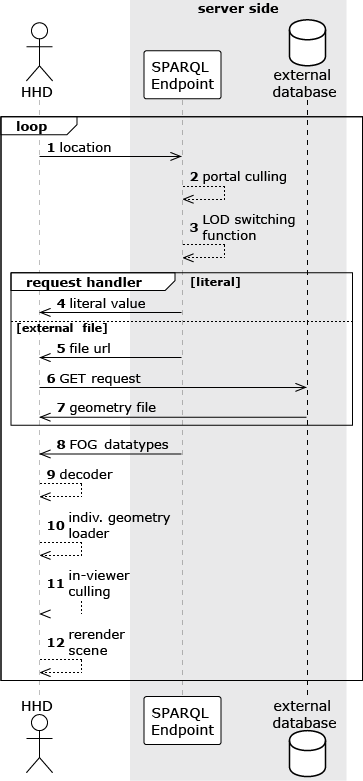
\includegraphics[width=6cm]{./figures/sequenceDiagram.png}
    \caption{Sequence diagram}
    \label{fig:sequendeDiagram}
\end{figure}
\section{Framework}
\subsection{Nextjs}
\section{Querying}
\subsection{Front-end}
\subsection{Back-end}
\section{Rendering}
\subsection{Xeokit \acs{sdk}}
The Xeokit \ac{sdk} ...


% \appendix
% \chapter{First appendix}
this is my first appendix
\clearpage
\chapter*{List of Acronyms}
\begin{acronym}[JSONP]\itemsep2pt\hypersetup{hidelinks}
  \acro{aec}[AEC]{Architecture, Engineering and Construction}  
  \acro{ar}[AR]{Augmented Reality}
  \acro{ascii}[ASCII]{American Standard Code for Information Interchange}
  \acro{bcf}[BCF]{\acs{bim} Collaboration Format}
  \acro{bcfowl}[bcfOWL]{\acs{bim} Collaboration Format Ontology}
  \acro{bim}[BIM]{Building Information Modelling}
  \acro{bot}[BOT]{Building Topology Ontology}
  \acro{bvh}[BVH]{Bounding Volume Hierarchy}
  \acro{chc}[CHC]{Coherent Hierarchical Culling algorithm}
  \acro{cpu}[CPU]{Central Processing Unit}
  \acro{dc}[DC]{Drop Culling}
  \acro{fog}[FOG]{File Ontology for Geometry formats}
  \acro{gis}[GIS]{Geographic Information System}
  \acro{gltf}[GLTF]{GL Transmission Format}
  \acro{gml}[GML]{Geography Markup Language}
  \acro{gpu}[GPU]{Graphics Processing Unit}
  \acro{hagi}[HAGI]{Hardware Accelerated Geometry Instancing}
  \acro{hhd}[HHD]{Hand Held Device}
  \acro{ifc}[IFC]{Industry Foundation Classes}
  \acro{ifcowl}[ifcOWL]{Industry Foundation Classes Ontology}
  \acro{json}[JSON]{JavaScript Object Notation}
  \acro{lbd-cg}[LBD-CG]{Linked Building Data Community Group}
  \acro{ldbim}[LDBIM]{Linked Data \acs{bim}}
  \acro{lod}[LOD]{Level of Detail}
  \acro{mep}[MEP]{Mechanical, Electrical and Plumbing}
  \acro{nohc}[NOHC]{Near Optimal Hierarchical Culling}
  \acro{oc}[OC]{Occlusion Culling}
  \acro{ogc}[OGC]{Open Geospatial Consortium}
  \acro{omg}[OMG]{Object Management Group}
  \acro{owl}[OWL]{Web Ontology Language}
  \acro{ram}[RAM]{Random Access Memory}
  \acro{rdf}[RDF]{Resource Description Framework}
  \acro{rdfs}[RDFS]{Resource Description Framework Schema}
  \acro{sdk}[SDK]{Software Development Kit}
  \acro{sparql}[SPARQL]{SPARQL Protocol and \acs{rdf} Query Language}
  \acro{sql}[SQL]{Structured Query Language}
  \acro{ui}[UI]{User Interface}
  \acro{uml}[UML]{Unified Modelling Language}
  \acro{uri}[URI]{Uniform Resource Identifier}
  \acro{vfc}[VFC]{View Frustum Culling}
  \acro{vram}[VRAM]{Video Random Access Memory}
  \acro{w3c}[W3C]{World Wide Web Consortium}
  \acro{wkt}[WKT]{Well-Known Text}
  \acro{xml}[XML]{Extensible Markup Language}
  \acro{xsd}[XSD]{\ac{xml} Schema Definition}
\end{acronym}

\printbibliography[nottype=web_page, heading=bibintoc,title={References}]
\printbibliography[type=web_page, heading=bibintoc, title={Referenced webistes}]
\end{document}
